\documentclass[10pt,journal]{IEEEtran}

\usepackage{graphicx}
\usepackage{amsmath}
\usepackage{amssymb}
\usepackage{booktabs}
\usepackage{hyperref}
\usepackage{multirow}
\usepackage{float}
\usepackage[font=small]{caption}

\graphicspath{{figures/}{../results/}}

\begin{document}

\title{Music Genre Classification Using Traditional Machine Learning and Convolutional Neural Networks: A Comparative Study on the GTZAN Dataset}

\author{Joshua~Oseimobor~(202492785),
        Covenant~Akisanmi~(202582097),
        and~Cletus~Chiemerie~(202492457)\\
        COMP-6915: Machine Learning, Winter 2026\\
        Memorial University of Newfoundland}

\maketitle

% ============================================================
\begin{abstract}
Music genre classification is a fundamental task in music information retrieval, enabling automated organization and recommendation of digital music libraries.
This paper presents a comparative study of traditional machine learning models---Support Vector Machine (SVM) and Random Forest---against a Convolutional Neural Network (CNN) for classifying audio signals into ten genres using the GTZAN dataset.
We extract a set of 57 hand-crafted audio features (MFCCs, spectral centroid, chroma, zero crossing rate, among others) for the traditional models and train a four-block CNN on log-mel spectrograms derived from three-second audio segments.
To ensure a fair comparison, all models are evaluated on the same track-level test set using stratified splits that prevent data leakage between segments of the same track.
We further investigate feature discriminability through importance analysis using both Gini impurity and permutation-based methods, and assess model robustness under varying levels of additive Gaussian noise at five signal-to-noise ratios.
Our results show that the CNN with majority voting achieves the highest test accuracy of 78.7\%, followed by the SVM at 72.0\% and Random Forest at 67.3\%. The CNN also demonstrates superior noise robustness, retaining 32.0\% accuracy at 5~dB SNR compared to 20.7\% for SVM and 24.0\% for Random Forest.
Feature importance analysis reveals that chroma STFT statistics, perceptual feature variance, and mid-range MFCCs are the most discriminative across both traditional models.
We additionally develop a web-based demonstration application that allows real-time genre prediction on user-uploaded audio files.
\end{abstract}

\begin{IEEEkeywords}
Music genre classification, GTZAN, convolutional neural networks, support vector machines, random forests, mel-spectrogram, audio features, noise robustness.
\end{IEEEkeywords}

% ============================================================
\section{Introduction}

The rapid growth of digital music databases and streaming platforms has made automated music genre classification (MGC) an essential task for content organization, recommendation systems, and music information retrieval (MIR)~\cite{fu2011survey}. Platforms such as Spotify, Apple Music, and YouTube Music host catalogs containing tens of millions of tracks. Manual tagging of musical genres is inherently subjective, labor-intensive, and incapable of scaling to the volume of new content uploaded daily. Automating this process through machine learning enables platforms to organize libraries efficiently and deliver personalized listening experiences.

Genre classification is challenging because genre boundaries are inherently fuzzy and culturally dependent~\cite{muller2011signal}. A single track may exhibit characteristics of multiple genres---for instance, country rock blends elements of both country and rock, while jazz fusion borrows from jazz, funk, and electronic music. This ambiguity is reflected in low inter-annotator agreement rates observed in music tagging studies. Furthermore, audio signals are high-dimensional temporal data, requiring careful feature engineering or representation learning to extract musically meaningful patterns.

The GTZAN dataset~\cite{tzanetakis2002musical}, often referred to as the ``MNIST of sounds,'' has served as a standard benchmark for MGC research for over two decades. Despite its relatively small size (1,000 tracks across 10 genres), it continues to be widely used for comparative studies due to its accessibility and well-understood characteristics~\cite{sturm2013gtzan}. The dataset provides a controlled environment for evaluating the relative strengths of different modeling approaches without the confounding factors introduced by larger, noisier datasets.

A central question in audio classification is whether traditional feature-engineered models can match or exceed the performance of deep learning architectures on moderately-sized datasets. While CNNs have demonstrated remarkable success in large-scale audio tasks~\cite{hershey2017cnn}, the limited size of GTZAN may favor models with stronger inductive biases derived from domain-specific features. Understanding this tradeoff has practical implications for deployment scenarios where computational resources are limited or labeled data is scarce.

Beyond raw accuracy, the robustness of a classifier to real-world noise conditions is critical for practical deployment. Music recordings encountered in the wild may contain background noise, compression artifacts, or recording imperfections that degrade signal quality. Evaluating how gracefully models degrade under noise provides insight into their suitability for real-world applications.

This paper makes the following contributions:
\begin{enumerate}
    \item A rigorous comparative study between SVM, Random Forest, and CNN classifiers, with track-level data splitting to prevent leakage from augmented segments.
    \item A comprehensive feature importance analysis identifying which audio descriptors contribute most significantly to genre discrimination, using both Gini impurity and permutation importance methods.
    \item A noise robustness evaluation measuring how each model degrades under synthetic additive noise at multiple signal-to-noise ratios ranging from 40~dB to 5~dB.
    \item A web-based demonstration application enabling real-time genre classification of user-uploaded audio files.
\end{enumerate}

The remainder of this paper is organized as follows: Section~II reviews related work, Section~III describes the dataset and preprocessing pipeline, Section~IV details the modeling methodology, Section~V presents experimental results, Section~VI discusses findings and limitations, and Section~VII concludes with directions for future work.

% ============================================================
\section{Related Work}

\subsection{Feature-Based Audio Classification}

Early approaches to MGC relied on hand-crafted audio features. Tzanetakis and Cook~\cite{tzanetakis2002musical} introduced the GTZAN dataset and proposed the use of timbral features (spectral centroid, spectral rolloff, zero crossing rate), rhythmic content, and pitch-based features for genre classification, achieving approximately 61\% accuracy with Gaussian mixture models. Mel-Frequency Cepstral Coefficients (MFCCs), originally developed for speech recognition~\cite{davis1980comparison, logan2000mel}, have become the most widely adopted feature representation for music classification tasks due to their ability to compactly represent the spectral envelope of audio signals in a perceptually motivated frequency scale.

Subsequent work has explored combinations of multiple feature families. Li et al.~\cite{li2003automatic} demonstrated that ensemble methods combining spectral, temporal, and timbral feature sets can improve classification accuracy over single-feature approaches. Panagakis et al.~\cite{panagakis2009music} explored tensor factorization methods for combining multiple feature views. Nanni et al.~\cite{nanni2016combining} showed that fusing visual texture features extracted from spectrogram images with traditional acoustic descriptors yielded consistent improvements across multiple datasets.

\subsection{Traditional Machine Learning for MGC}

Support Vector Machines have been extensively applied to MGC, leveraging their effectiveness in high-dimensional feature spaces~\cite{cortes1995support}. The RBF kernel is particularly popular because it can model non-linear decision boundaries in the feature space without explicit feature mapping. Random Forests~\cite{breiman2001random} offer complementary advantages: they provide natural feature importance rankings through Gini impurity, are robust to overfitting on noisy features, and require minimal hyperparameter tuning. Both classifiers benefit from careful feature standardization and cross-validated hyperparameter selection.

\subsection{Deep Learning Approaches}

The application of CNNs to audio classification reframes the problem as image recognition on spectrogram representations~\cite{costa2017evaluation}. This approach has the advantage of learning hierarchical feature representations directly from the data, potentially discovering patterns that hand-crafted features miss. Choi et al.~\cite{choi2017convolutional} introduced convolutional recurrent architectures that capture both local spectral patterns and longer-range temporal dynamics. Dieleman and Schrauwen~\cite{dieleman2014end} explored end-to-end learning directly from raw waveforms, bypassing explicit feature extraction entirely.

Hershey et al.~\cite{hershey2017cnn} conducted a systematic comparison of CNN architectures for large-scale audio classification, finding that deeper architectures with batch normalization and residual connections achieved the best results. Lidy and Schindler~\cite{lidy2016parallel} proposed parallel CNN architectures that process mel-spectrograms at multiple temporal resolutions simultaneously. These studies suggest that architectural choices---including normalization, regularization, and pooling strategies---play a crucial role in CNN performance on audio tasks.

\subsection{Data Augmentation for Audio}

Data augmentation is particularly important for small audio datasets like GTZAN. Park et al.~\cite{park2019specaugment} proposed SpecAugment, a simple augmentation method that applies frequency masking and time masking directly to log-mel spectrograms. Originally developed for automatic speech recognition, SpecAugment has been shown to improve generalization without introducing any additional training data. We adopt a similar strategy for our CNN training, applying random frequency and time masks during the training phase.

\subsection{GTZAN Dataset Limitations and Evaluation Practices}

Sturm~\cite{sturm2013gtzan} conducted a thorough audit of the GTZAN dataset, documenting several faults including mislabeled tracks, exact repetitions, and a truncated file (\texttt{jazz.00054.wav}). Critically, Sturm also highlighted the importance of track-level splitting: because many studies split data at the segment or frame level, segments from the same track can appear in both training and test sets, artificially inflating reported accuracies. Our pipeline explicitly handles these known issues through validation, exclusion of corrupted files, and strict track-level partitioning.

% ============================================================
\section{Dataset and Preprocessing}

\subsection{GTZAN Dataset}
The GTZAN dataset contains 1,000 audio tracks, each 30 seconds long, evenly distributed across 10 genres: blues, classical, country, disco, hip-hop, jazz, metal, pop, reggae, and rock. All files are mono WAV format sampled at 22,050~Hz with 16-bit depth. The dataset represents a balanced classification problem with 100 tracks per genre.

\subsection{Data Validation}
We perform automated validation of all audio files, checking for duration consistency and loading integrity using the librosa library~\cite{mcfee2015librosa}. Each file is loaded and its duration is verified against the expected 30-second length. One known corrupted file (\texttt{jazz.00054.wav}, which is truncated to approximately 91\% of its expected duration at roughly 27.4 seconds) is automatically detected and excluded, leaving 999 valid tracks for all subsequent experiments.

\subsection{Data Augmentation via Segmentation}
Each 30-second track is segmented into ten non-overlapping 3-second clips, expanding the effective dataset from 999 tracks to 9,990 audio segments. Each segment corresponds to $3 \times 22{,}050 = 66{,}150$ audio samples. This segmentation provides sufficient training data for the CNN while maintaining manageable computational requirements. Importantly, segments from the same track are never split across different data partitions.

\subsection{Train/Validation/Test Split}
To prevent data leakage, all splits are performed at the \textbf{track level} before segmentation. We use a 70/15/15 stratified split, yielding 699 training tracks (6,990 segments), 150 validation tracks (1,500 segments), and 150 test tracks (1,500 segments). Stratification ensures equal genre proportions across all three partitions. This strict track-level separation prevents the model from memorizing recording-specific characteristics (room acoustics, microphone quality, mastering style) rather than learning genuine genre-level patterns.

% ============================================================
\section{Methods}

\subsection{Feature Extraction for Traditional Models}

For the traditional ML models, we extract a comprehensive set of 57 audio features per 30-second track from the GTZAN-provided CSV file. Table~\ref{tab:features} summarizes the feature categories.

\begin{table}[ht]
\centering
\caption{Audio features extracted for traditional ML models.}
\label{tab:features}
\begin{tabular}{@{}lcc@{}}
\toprule
\textbf{Feature Category} & \textbf{Descriptors} & \textbf{Count} \\
\midrule
Chroma STFT & mean, variance & 2 \\
RMS Energy & mean, variance & 2 \\
Spectral Centroid & mean, variance & 2 \\
Spectral Bandwidth & mean, variance & 2 \\
Spectral Rolloff & mean, variance & 2 \\
Zero Crossing Rate & mean, variance & 2 \\
Harmony & mean, variance & 2 \\
Perceptual & mean, variance & 2 \\
Tempo & single value & 1 \\
MFCCs (1--20) & mean, variance each & 40 \\
\midrule
\textbf{Total} & & \textbf{57} \\
\bottomrule
\end{tabular}
\end{table}

MFCCs capture the spectral envelope shape through a series of cosine transforms applied to the log-mel spectrum~\cite{davis1980comparison}. The first few coefficients represent overall spectral shape (brightness, energy distribution), while higher-order coefficients capture finer spectral details. Spectral centroid indicates the ``center of gravity'' of the spectrum and correlates with perceived brightness. Zero crossing rate approximates the dominant frequency content and distinguishes noisy from harmonic signals.

All features are standardized using a \texttt{StandardScaler} fitted exclusively on the training set to prevent information leakage from validation or test statistics. The same fitted scaler is applied to both validation and test partitions.

\subsection{Mel-Spectrogram Generation for CNN}

For the CNN, we compute log-mel spectrograms from each 3-second audio segment. The computation pipeline is as follows:
\begin{enumerate}
    \item Load the 3-second audio segment (66,150 samples at 22,050~Hz).
    \item Compute the Short-Time Fourier Transform with a window size of 2,048 samples (approximately 93~ms) and a hop length of 512 samples (approximately 23~ms).
    \item Apply a bank of 128 mel-scaled triangular filters to obtain the mel spectrogram.
    \item Convert to log scale: $S_{\text{log}} = \log(S_{\text{mel}} + \epsilon)$ where $\epsilon = 10^{-10}$.
    \item Normalize each spectrogram to the range $[0, 1]$.
\end{enumerate}
The resulting spectrogram has dimensions $128 \times 130$ (frequency bins $\times$ time frames) and is treated as a single-channel image input to the CNN.

\subsection{Support Vector Machine}

We train an SVM classifier~\cite{cortes1995support} with hyperparameter optimization via 5-fold stratified cross-validated grid search. The search space includes: regularization parameter $C \in \{0.1, 1, 10, 100\}$, kernel type $\in \{\text{RBF}, \text{linear}\}$, and kernel coefficient $\gamma \in \{\text{scale}, \text{auto}\}$. The scoring metric is macro-averaged F1-score, which weights all genres equally regardless of potential class imbalance. The best configuration found is $C = 100$, kernel = RBF, and $\gamma = \text{scale}$, achieving a cross-validation macro F1 of 0.561.

\subsection{Random Forest}

We train a Random Forest classifier~\cite{breiman2001random} with 5-fold stratified cross-validated grid search over: $n_{\text{estimators}} \in \{100, 200, 500\}$, $\text{max\_depth} \in \{10, 20, 30, \text{None}\}$, and $\text{min\_samples\_split} \in \{2, 5\}$. The best configuration found is $n_{\text{estimators}} = 100$, $\text{max\_depth} = \text{None}$ (unlimited), and $\text{min\_samples\_split} = 5$, achieving a cross-validation macro F1 of 0.543. The unlimited depth allows the Random Forest to fully grow its trees, relying on the ensemble averaging to control variance.

\subsection{Convolutional Neural Network}

We design a four-block CNN architecture (Figure~\ref{fig:cnn_arch}) that processes single-channel mel-spectrograms of shape $128 \times 130 \times 1$. Table~\ref{tab:cnn_arch} details the layer configuration and parameter count.

\begin{figure}[ht]
\centering
\fbox{\parbox{0.9\linewidth}{\small
\textbf{Input:} $128 \times 130 \times 1$ \\[4pt]
$\rightarrow$ Conv2D(32, 3$\times$3) $\rightarrow$ BN $\rightarrow$ ReLU $\rightarrow$ MaxPool(2$\times$2) $\rightarrow$ Drop(0.3) \\
$\rightarrow$ Conv2D(64, 3$\times$3) $\rightarrow$ BN $\rightarrow$ ReLU $\rightarrow$ MaxPool(2$\times$2) $\rightarrow$ Drop(0.3) \\
$\rightarrow$ Conv2D(128, 3$\times$3) $\rightarrow$ BN $\rightarrow$ ReLU $\rightarrow$ MaxPool(2$\times$2) $\rightarrow$ Drop(0.3) \\
$\rightarrow$ Conv2D(256, 3$\times$3) $\rightarrow$ BN $\rightarrow$ ReLU $\rightarrow$ MaxPool(2$\times$2) $\rightarrow$ Drop(0.3) \\[4pt]
$\rightarrow$ GlobalAvgPool $\rightarrow$ Dense(256) $\rightarrow$ BN $\rightarrow$ ReLU $\rightarrow$ Drop(0.5) \\
$\rightarrow$ Dense(10, softmax) \\[4pt]
\textbf{Output:} 10-class probability distribution \\
\textbf{Total parameters:} 459,146
}}
\caption{CNN architecture for mel-spectrogram classification.}
\label{fig:cnn_arch}
\end{figure}

\begin{table}[ht]
\centering
\caption{CNN layer configuration and output shapes.}
\label{tab:cnn_arch}
\begin{tabular}{@{}lcc@{}}
\toprule
\textbf{Layer} & \textbf{Output Shape} & \textbf{Params} \\
\midrule
Input          & $128 \times 130 \times 1$ & 0 \\
Conv Block 1   & $64 \times 65 \times 32$  & 416 \\
Conv Block 2   & $32 \times 32 \times 64$  & 18,560 \\
Conv Block 3   & $16 \times 16 \times 128$ & 73,984 \\
Conv Block 4   & $8 \times 8 \times 256$   & 295,424 \\
Global Avg Pool & $256$                    & 0 \\
Dense + BN     & $256$                     & 66,304 \\
Output Dense   & $10$                      & 2,570 \\
\midrule
\textbf{Total} & & \textbf{459,146} \\
\bottomrule
\end{tabular}
\end{table}

Key design choices include:
\begin{itemize}
    \item \textbf{Batch Normalization}~\cite{ioffe2015batch} after each convolutional layer to stabilize training and enable higher learning rates.
    \item \textbf{Progressive Dropout}~\cite{srivastava2014dropout} at 0.3 after each pooling layer and 0.5 before the final classification layer, combined with L2 regularization ($\lambda = 0.001$) on all convolutional kernel weights, to combat overfitting on the small dataset.
    \item \textbf{Global Average Pooling} instead of flattening, which reduces the parameter count significantly and acts as structural regularization by forcing each feature map to encode one discriminative pattern.
\end{itemize}

\subsection{CNN Training Procedure}

The model is trained using the Adam optimizer~\cite{kingma2014adam} with an initial learning rate of $10^{-3}$. We employ two callbacks to manage training dynamics:
\begin{itemize}
    \item \textbf{ReduceLROnPlateau}: Reduces the learning rate by a factor of 0.5 when validation loss plateaus for 5 consecutive epochs, with a minimum learning rate of $10^{-6}$.
    \item \textbf{EarlyStopping}: Stops training after 10 epochs without improvement in validation loss, restoring the weights from the best epoch.
\end{itemize}

During training, we apply SpecAugment-style augmentation~\cite{park2019specaugment}, randomly masking up to 15 consecutive frequency bands and up to 10 consecutive time frames in each spectrogram. This augmentation is applied on-the-fly during training only, not during validation or testing.

For track-level evaluation, the CNN classifies each of the 10 segments from a 30-second track independently, and the final genre prediction is determined by majority voting across all 10 segment-level predictions. In case of a tie, the class with the highest total predicted probability is selected. This ensures a fair comparison with the traditional models, which operate on full 30-second feature vectors.

\subsection{Noise Robustness Protocol}

To assess model robustness under realistic degradation conditions, we inject additive white Gaussian noise into the test set audio at signal-to-noise ratios (SNR) of 40, 30, 20, 10, and 5~dB. The noise is generated as:
\begin{equation}
x_{\text{noisy}} = x_{\text{clean}} + \alpha \cdot n, \quad \alpha = \sqrt{\frac{P_{\text{signal}}}{10^{\text{SNR}/10}}}
\end{equation}
where $n \sim \mathcal{N}(0, 1)$ and $P_{\text{signal}}$ is the mean power of the clean signal. For each noise level, we re-extract all features (for SVM/RF) and regenerate mel-spectrograms (for CNN), then evaluate all models on the degraded data. This protocol directly answers our third research question regarding noise sensitivity and simulates conditions such as background noise in live recordings or low-quality audio captures.

% ============================================================
\section{Experiments and Results}

\subsection{Experimental Setup}

All experiments are conducted using Python 3.11 with scikit-learn~\cite{pedregosa2011scikit} for traditional ML, TensorFlow 2.21~\cite{tensorflow2015} for deep learning, and librosa~\cite{mcfee2015librosa} for audio processing. The random seed is fixed at 42 for reproducibility across all random operations including data splitting, weight initialization, and hyperparameter search. All training is performed on CPU to ensure reproducibility across different hardware configurations.

\subsection{Overall Model Comparison}

Table~\ref{tab:comparison} presents the classification performance of all three models on the held-out test set (150 tracks). The CNN with track-level majority voting achieves the highest accuracy at 78.7\%, outperforming the SVM (72.0\%) by 6.7 percentage points and the Random Forest (67.3\%) by 11.3 percentage points.

\begin{table}[ht]
\centering
\caption{Model performance comparison on the test set (150 tracks).}
\label{tab:comparison}
\begin{tabular}{@{}lccc@{}}
\toprule
\textbf{Model} & \textbf{Accuracy} & \textbf{F1 (Macro)} & \textbf{F1 (Weighted)} \\
\midrule
SVM             & 0.720 & 0.719 & 0.719 \\
Random Forest   & 0.673 & 0.667 & 0.667 \\
CNN (Maj. Vote) & \textbf{0.787} & \textbf{0.785} & \textbf{0.785} \\
\bottomrule
\end{tabular}
\end{table}

\subsection{Per-Class Analysis}

Table~\ref{tab:perclass} reports the per-genre F1-scores for the SVM and Random Forest classifiers. Both models demonstrate that classical music and hip-hop are among the easiest genres to classify, likely due to their distinctive spectral signatures---classical features prominent harmonic and tonal content with low percussive energy, while hip-hop exhibits characteristic low-frequency emphasis and rhythmic patterns.

\begin{table}[ht]
\centering
\caption{Per-genre F1-scores for traditional ML models.}
\label{tab:perclass}
\begin{tabular}{@{}lcccccc@{}}
\toprule
\textbf{Genre} & \multicolumn{3}{c}{\textbf{SVM}} & \multicolumn{3}{c}{\textbf{Random Forest}} \\
\cmidrule(lr){2-4} \cmidrule(lr){5-7}
 & P & R & F1 & P & R & F1 \\
\midrule
Blues     & 0.58 & 0.47 & 0.52 & 0.82 & 0.60 & 0.69 \\
Classical & 0.87 & 0.87 & 0.87 & 0.88 & 0.93 & 0.90 \\
Country   & 0.73 & 0.73 & 0.73 & 0.75 & 0.80 & 0.77 \\
Disco     & 0.73 & 0.73 & 0.73 & 0.47 & 0.47 & 0.47 \\
Hip-hop   & 0.78 & 0.93 & 0.85 & 0.52 & 0.73 & 0.61 \\
Jazz      & 0.72 & 0.87 & 0.79 & 0.75 & 0.80 & 0.77 \\
Metal     & 1.00 & 0.73 & 0.85 & 0.75 & 0.80 & 0.77 \\
Pop       & 0.67 & 0.53 & 0.59 & 0.75 & 0.80 & 0.77 \\
Reggae    & 0.50 & 0.67 & 0.57 & 0.67 & 0.53 & 0.59 \\
Rock      & 0.71 & 0.67 & 0.69 & 0.36 & 0.27 & 0.31 \\
\bottomrule
\end{tabular}
\end{table}

The SVM achieves perfect precision on metal (1.00) but lower recall (0.73), indicating conservative metal predictions that are highly reliable. Blues is the SVM's weakest genre (F1: 0.52), reflecting the stylistic overlap between blues, jazz, and rock. The Random Forest struggles most severely with rock (F1: 0.31), misclassifying rock tracks across several neighboring genres, and disco (F1: 0.47). Conversely, the Random Forest outperforms the SVM on blues (F1: 0.69 vs.\ 0.52).

The CNN with majority voting achieves particularly strong results on hip-hop (F1: 0.91), metal (F1: 0.93), and jazz (F1: 0.89), demonstrating its ability to identify distinctive spectral patterns in these genres. However, the CNN struggles most with country (recall: 0.40), where country tracks are misclassified across multiple genres including blues, rock, and pop---reflecting the genuine stylistic breadth of country music.

\begin{figure}[ht]
\centering
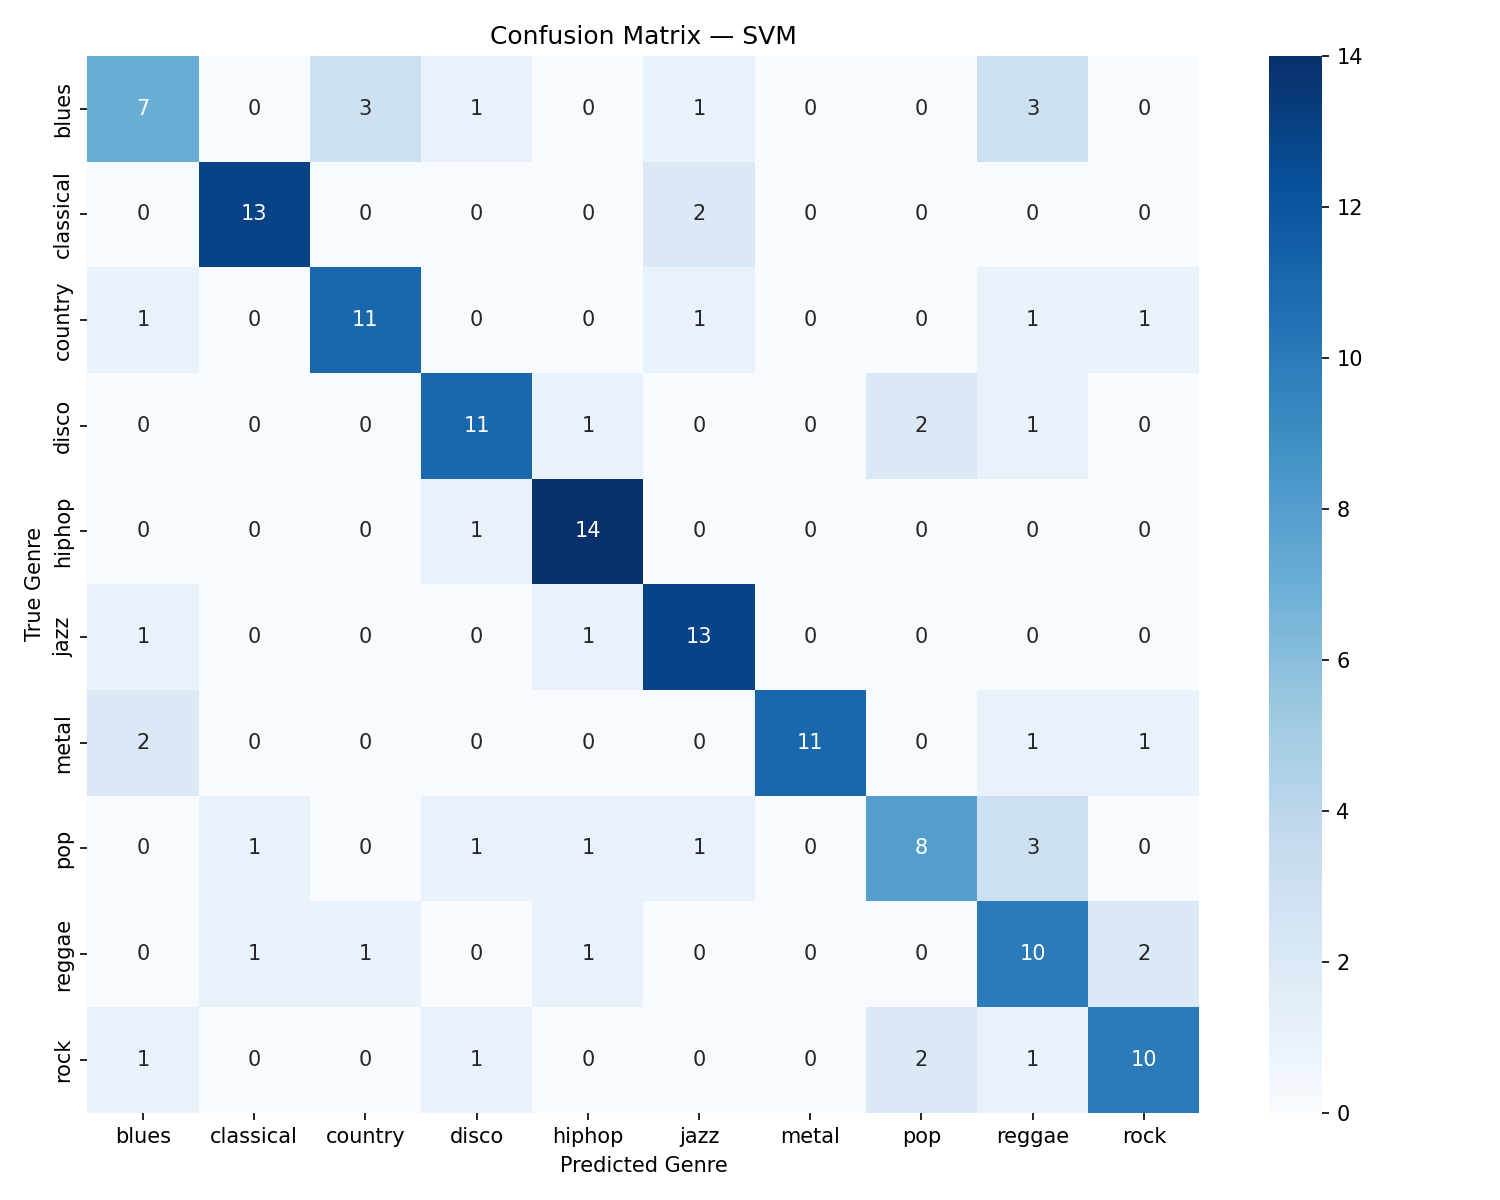
\includegraphics[width=\linewidth]{confusion_matrix_svm.png}
\caption{Confusion matrix for the SVM classifier.}
\label{fig:cm_svm}
\end{figure}

\begin{figure}[ht]
\centering
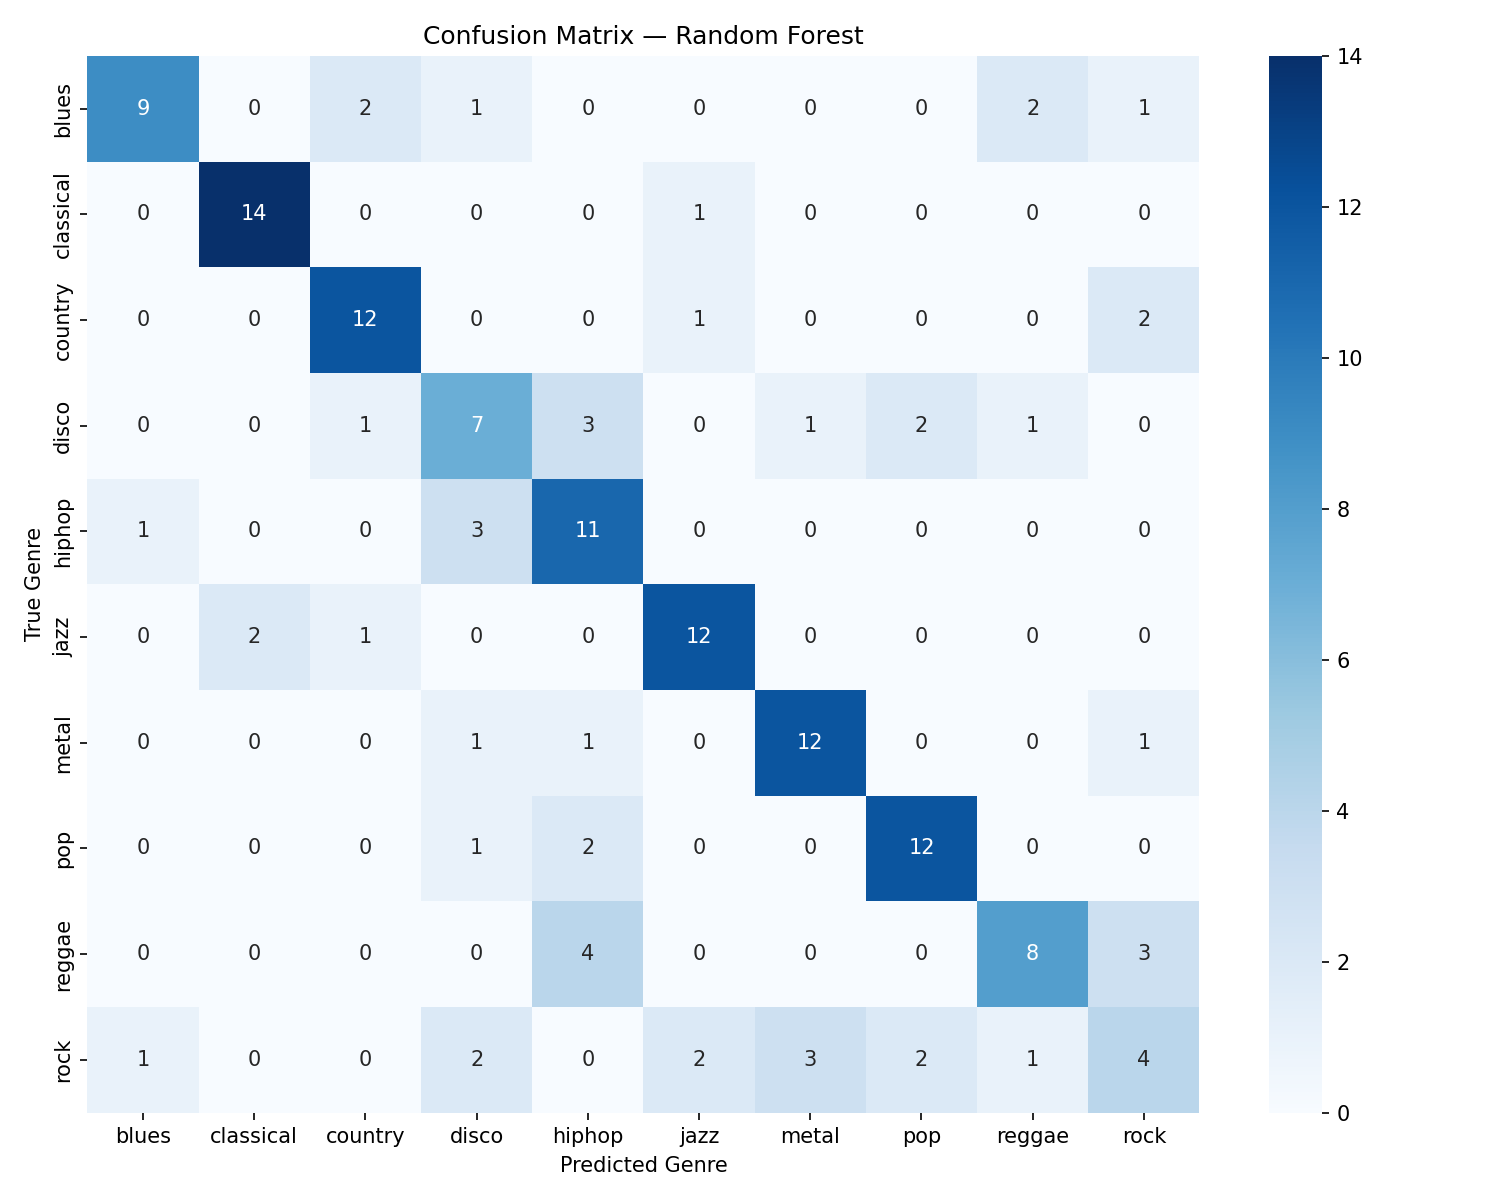
\includegraphics[width=\linewidth]{confusion_matrix_random_forest.png}
\caption{Confusion matrix for the Random Forest classifier.}
\label{fig:cm_rf}
\end{figure}

\begin{figure}[ht]
\centering
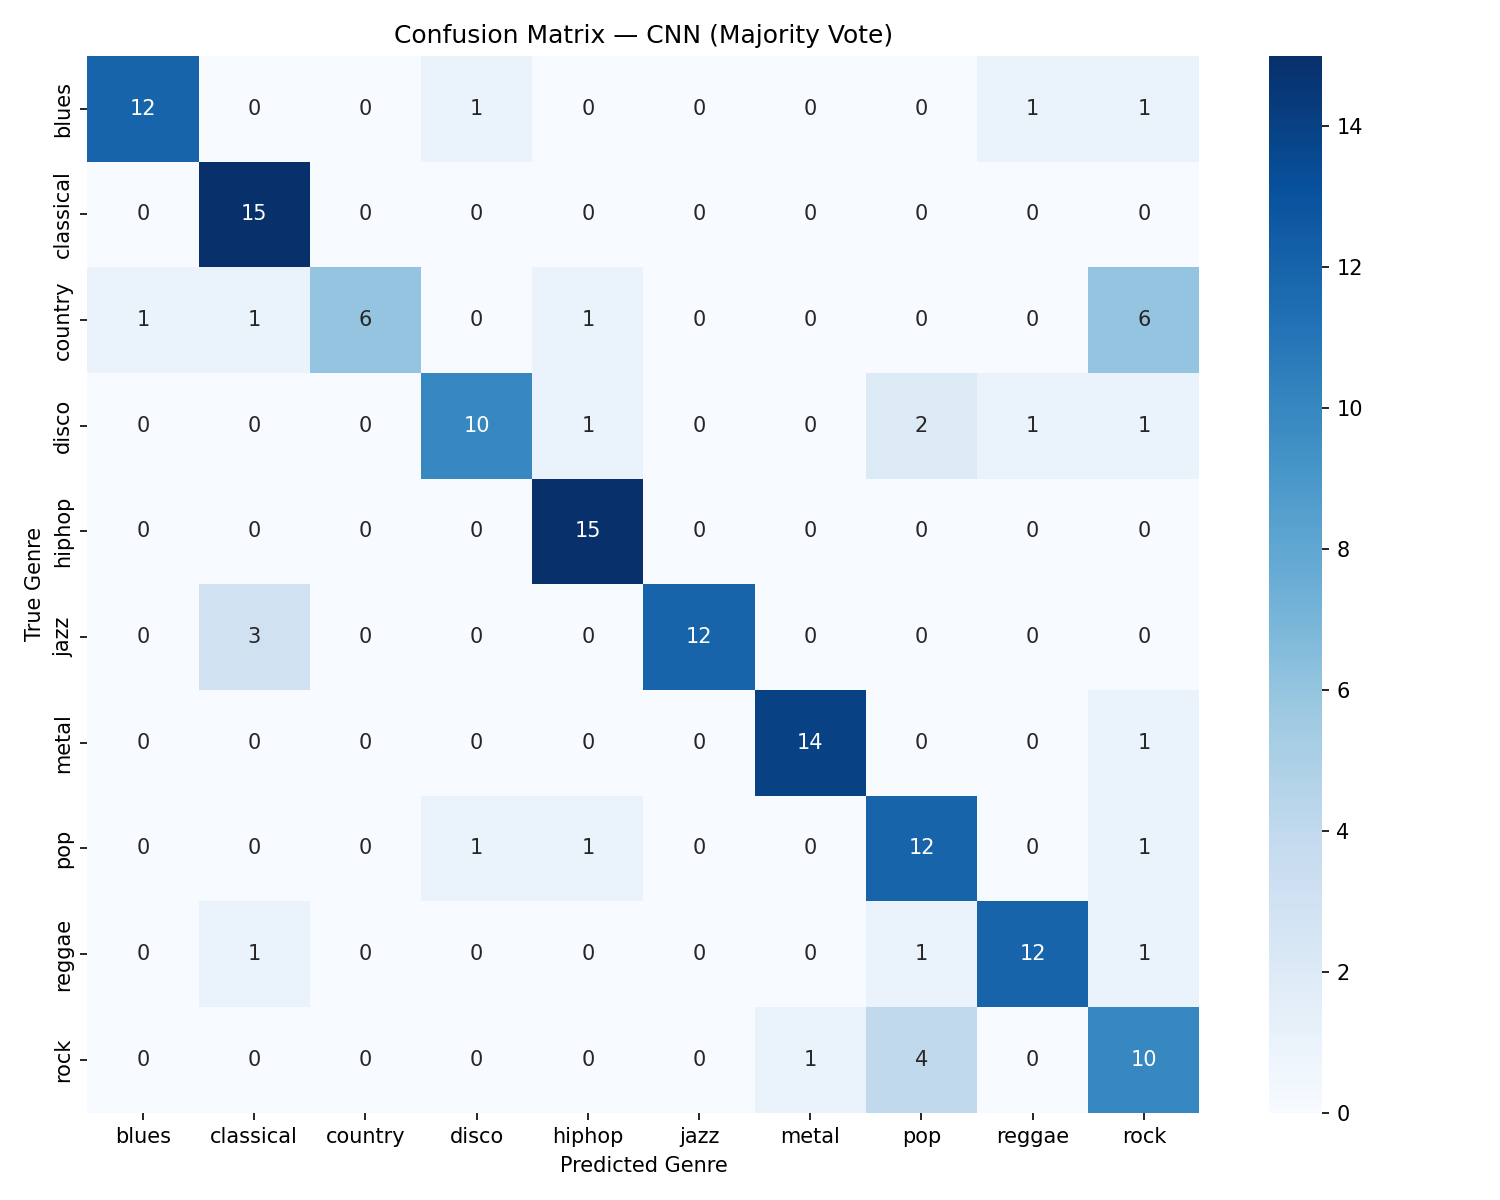
\includegraphics[width=\linewidth]{confusion_matrix_cnn_majority_vote.png}
\caption{Confusion matrix for the CNN classifier (majority vote).}
\label{fig:cm_cnn}
\end{figure}

The confusion matrices (Figures~\ref{fig:cm_svm}--\ref{fig:cm_cnn}) reveal systematic genre confusion patterns. Across all three models, rock is consistently the most confused genre, frequently misclassified as country, blues, or disco. The blues--jazz and country--rock confusion pairs appear prominently in all matrices, reflecting genuine musical similarities between these genre pairs. The CNN's confusion matrix shows more concentrated diagonal entries compared to the traditional models, indicating more confident and decisive classifications overall.

\subsection{CNN Training Dynamics}

Figure~\ref{fig:training_curves} shows the training and validation loss and accuracy curves over the course of CNN training. The model achieves its best validation loss of 0.908 at epoch 42, with a corresponding validation accuracy of 79.7\%. Early stopping triggers at epoch 52 after 10 consecutive epochs without improvement, and the best weights from epoch 42 are restored.

The training accuracy plateaus around 93\%, yielding a train--validation gap of approximately 13 percentage points. This moderate gap is typical for small datasets and indicates some degree of overfitting despite our multi-faceted regularization strategy (dropout, L2, batch normalization, SpecAugment). The \texttt{ReduceLROnPlateau} scheduler reduces the learning rate four times during training, from the initial $10^{-3}$ down to $3.125 \times 10^{-5}$, with each reduction corresponding to a brief improvement in validation metrics before the plateau resumes.

\begin{figure}[ht]
\centering
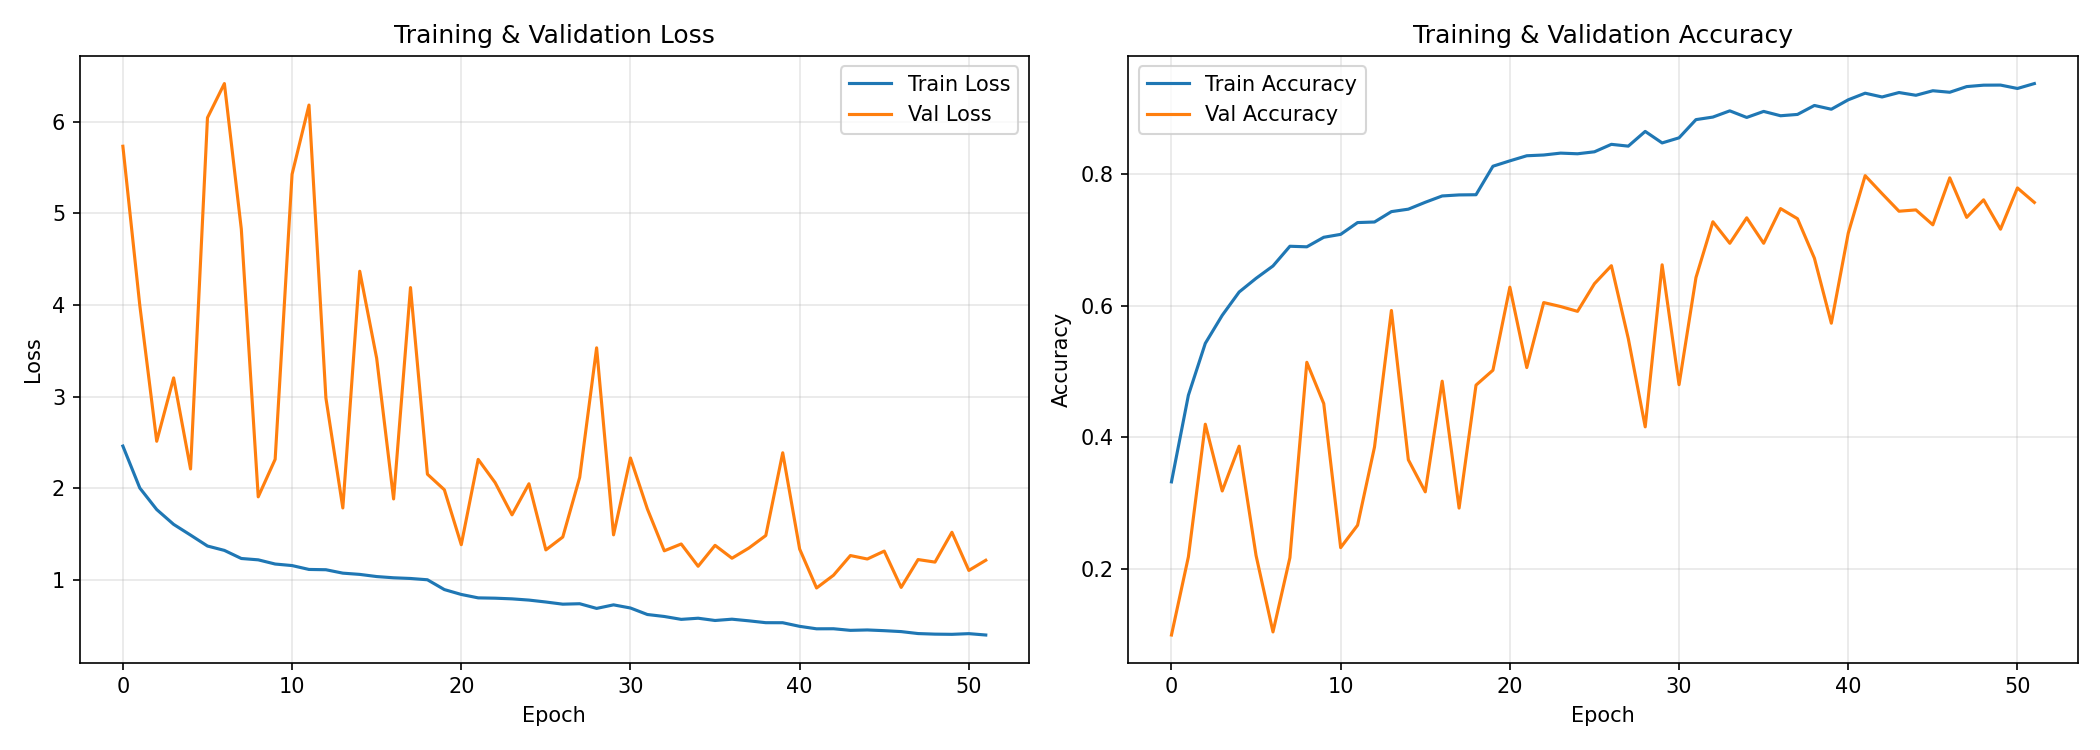
\includegraphics[width=\linewidth]{training_curves_cnn.png}
\caption{CNN training and validation loss/accuracy curves over 52 epochs.}
\label{fig:training_curves}
\end{figure}

\subsection{Feature Importance Analysis}

We analyze feature importance using two complementary methods: Gini impurity from the Random Forest and permutation importance from the SVM. Figure~\ref{fig:fi_rf} presents the top 20 features ranked by Gini importance.

The most discriminative feature according to the Random Forest is \texttt{chroma\_stft\_mean} (importance: 0.052), followed by \texttt{perceptr\_var} (0.045) and \texttt{chroma\_stft\_var} (0.038). Permutation importance analysis on the SVM reveals a different ranking, with \texttt{mfcc4\_mean} (0.052) and \texttt{mfcc11\_mean} (0.036) leading, though both methods agree on the importance of \texttt{perceptr\_var} and \texttt{chroma\_stft\_var}.

\begin{figure}[ht]
\centering
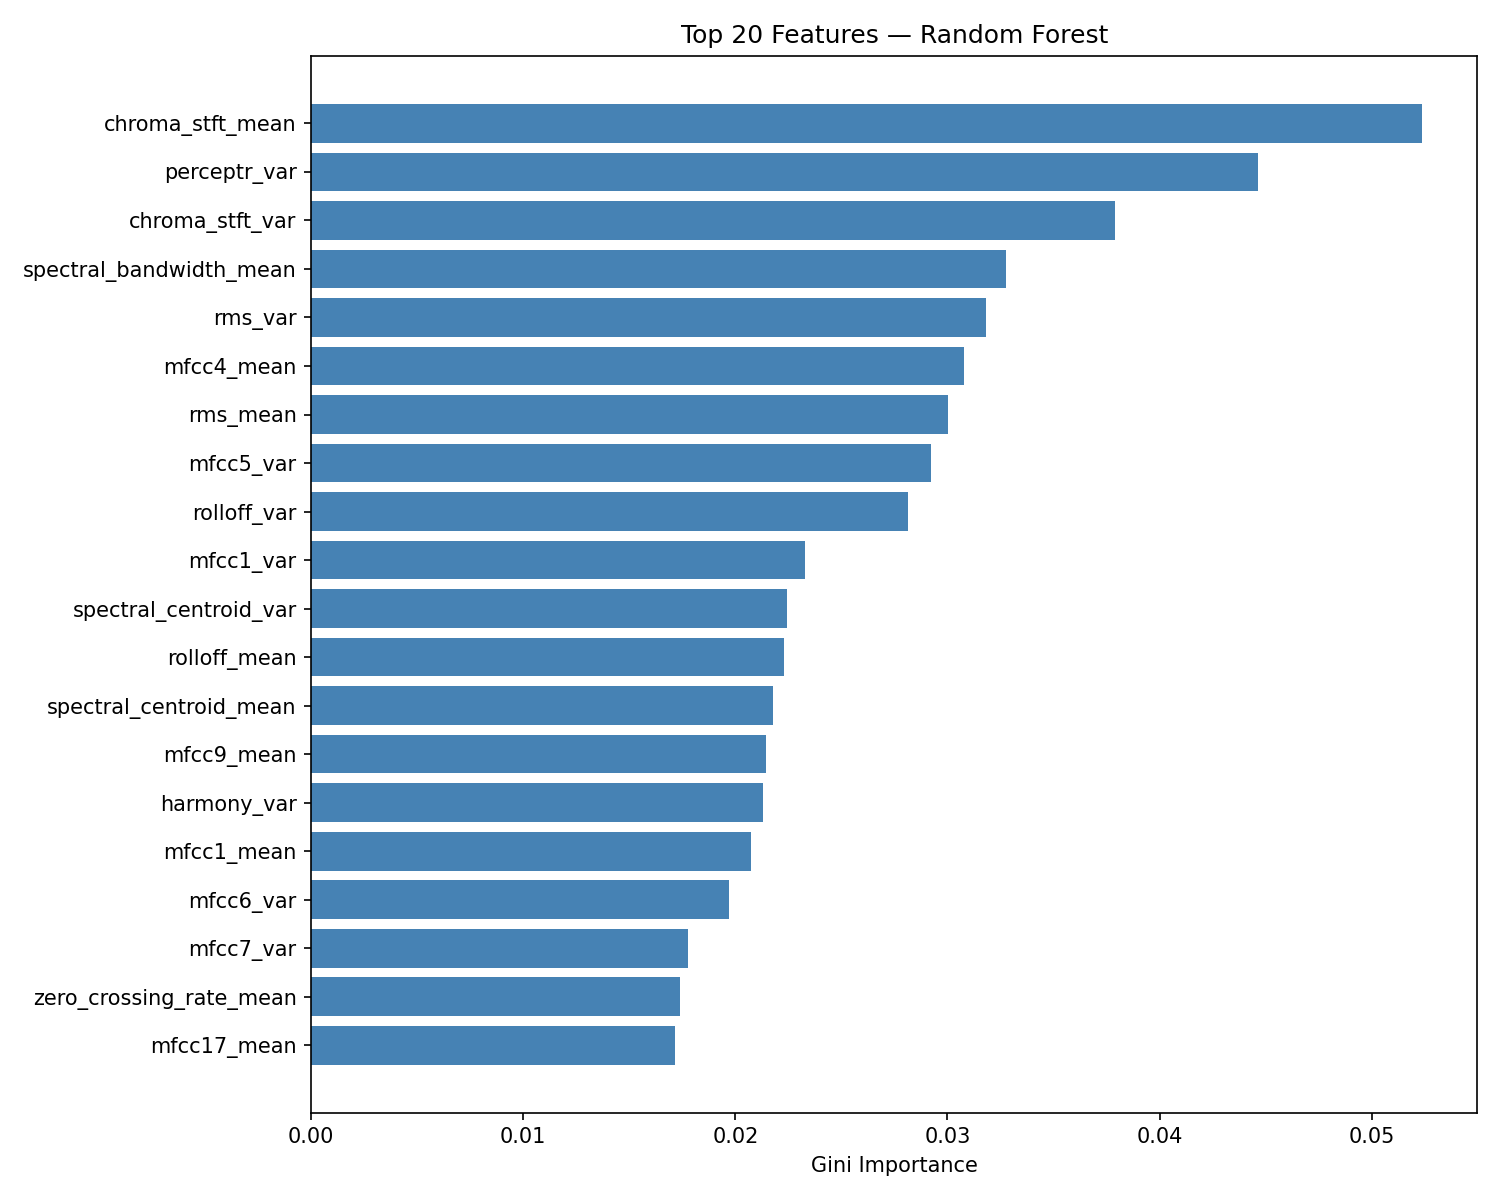
\includegraphics[width=\linewidth]{feature_importance_rf.png}
\caption{Top 20 features ranked by Gini importance (Random Forest).}
\label{fig:fi_rf}
\end{figure}

\begin{figure}[ht]
\centering
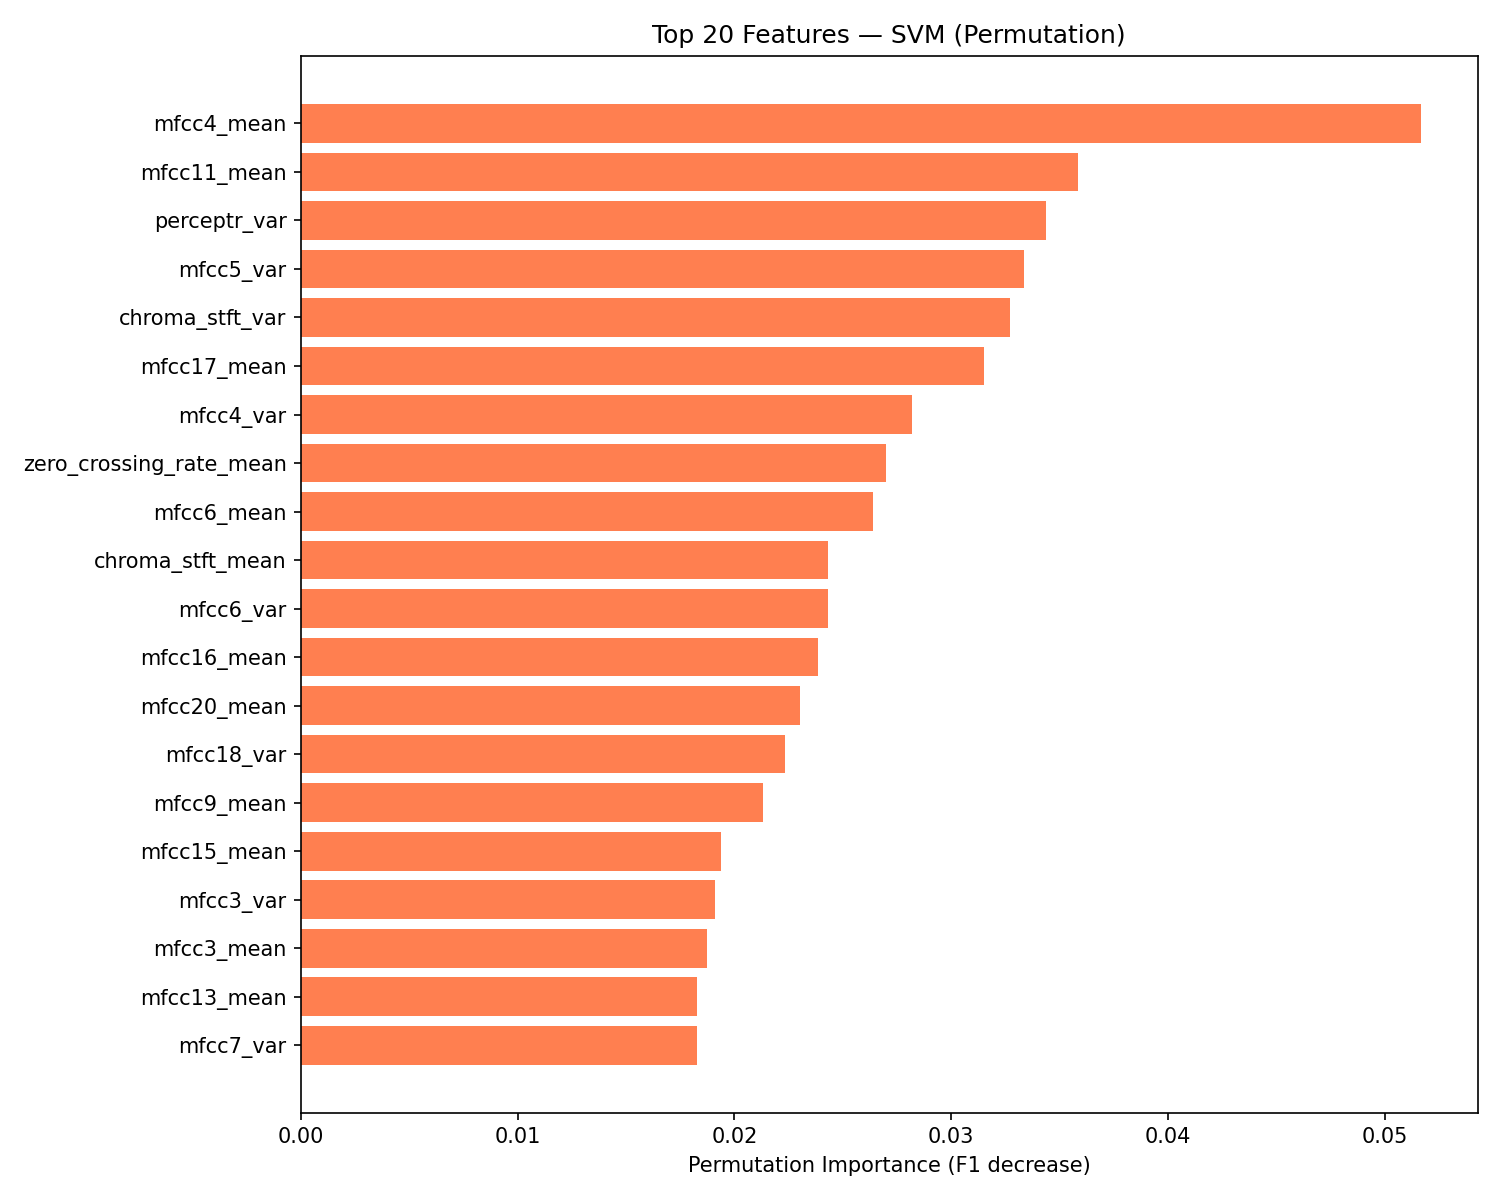
\includegraphics[width=\linewidth]{feature_importance_svm.png}
\caption{Top 20 features ranked by permutation importance (SVM).}
\label{fig:fi_svm}
\end{figure}

The consensus set of features appearing in both models' top~10 includes chroma STFT statistics, perceptual feature variance, several mid-range MFCC coefficients (4, 5, 6, 7, 9, 17), and zero crossing rate. The divergence between Gini and permutation importance rankings reflects the different ways these metrics capture feature relevance: Gini importance measures the average impurity decrease when splitting on a feature across all trees, while permutation importance measures the accuracy drop when a feature's values are randomly shuffled. The finding that mid-range MFCCs (coefficients 4--11) are more discriminative than the first few MFCCs is notable, as it suggests that fine-grained spectral texture, rather than gross spectral shape, is most informative for genre discrimination.

\subsection{Noise Robustness}

Figure~\ref{fig:noise} illustrates how each model's accuracy degrades under additive Gaussian noise at five SNR levels. Table~\ref{tab:noise} provides the exact accuracy values.

\begin{table}[ht]
\centering
\caption{Model accuracy (\%) at each noise level (SNR in dB).}
\label{tab:noise}
\begin{tabular}{@{}lccccc@{}}
\toprule
\textbf{Model} & \textbf{40 dB} & \textbf{30 dB} & \textbf{20 dB} & \textbf{10 dB} & \textbf{5 dB} \\
\midrule
SVM           & 70.0 & 60.0 & 40.0 & 25.3 & 20.7 \\
Random Forest & 67.3 & 56.7 & 39.3 & 28.0 & 24.0 \\
CNN           & \textbf{78.7} & \textbf{64.0} & \textbf{52.0} & \textbf{39.3} & \textbf{32.0} \\
\bottomrule
\end{tabular}
\end{table}

At 40~dB (minimal noise), all models retain near-clean performance, confirming that mild noise has negligible impact. At 20~dB, a moderate noise level comparable to a moderately noisy room, the CNN retains 52.0\% accuracy compared to 40.0\% for SVM and 39.3\% for Random Forest. Under severe noise at 5~dB, the CNN still achieves 32.0\% accuracy (well above the 10\% random baseline), while SVM drops to 20.7\% and Random Forest to 24.0\%.

\begin{figure}[ht]
\centering
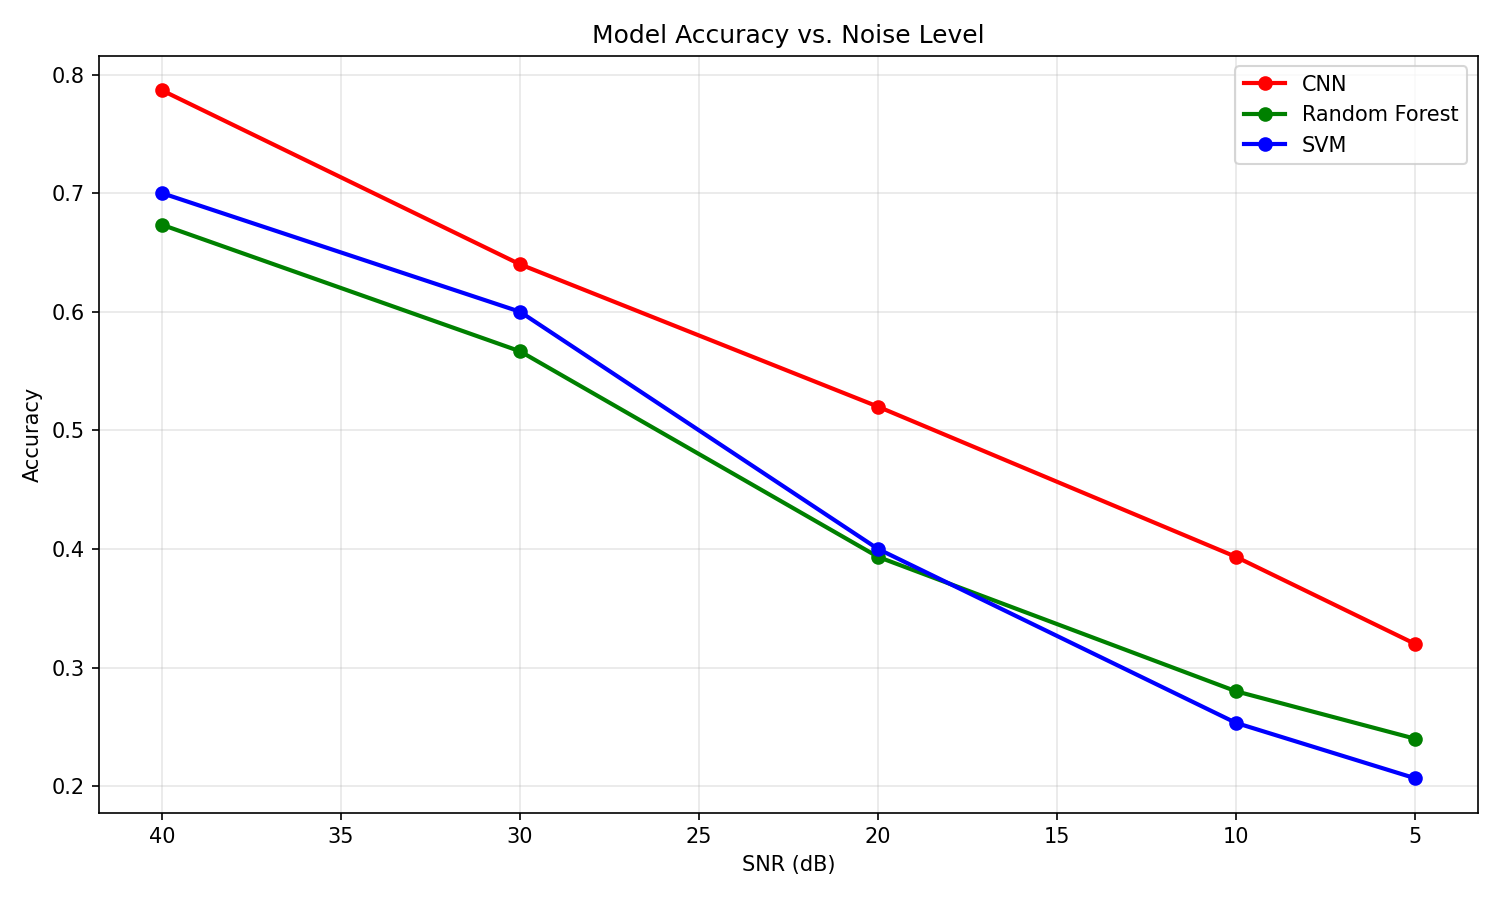
\includegraphics[width=\linewidth]{noise_robustness.png}
\caption{Model accuracy as a function of signal-to-noise ratio (dB).}
\label{fig:noise}
\end{figure}

The CNN's superior noise resilience is consistent across all noise levels, maintaining an average advantage of approximately 10 percentage points over SVM. This resilience likely stems from the CNN's learned spectral representations, which can capture robust spatial patterns in mel-spectrograms even when noise corrupts individual frequency bands. In contrast, the hand-crafted statistical features used by SVM and Random Forest (particularly spectral moments and zero crossing rate) are directly impacted by broadband additive noise, which shifts their values away from clean-signal distributions.

Interestingly, the Random Forest slightly outperforms the SVM at higher noise levels (28.0\% vs.\ 25.3\% at 10~dB, and 24.0\% vs.\ 20.7\% at 5~dB), despite underperforming on clean data. This may be because the ensemble averaging in Random Forest provides inherent noise smoothing through its bagging procedure, whereas the SVM's decision boundaries are more sensitive to feature perturbations.

% ============================================================
\section{Discussion}

\subsection{Genre Confusion Patterns}

The confusion matrices reveal systematic patterns that reflect genuine musical relationships. Rock is consistently the most difficult genre across all three models, frequently confused with country, blues, and disco. This reflects the broad stylistic diversity within rock music---from soft acoustic rock (which overlaps with country and folk) to hard rock (which overlaps with metal) to classic rock (which shares heritage with blues). Conversely, classical and metal are classified with high precision by all models, likely due to their distinctive spectral characteristics: classical music features prominently harmonic tonal content with minimal percussive elements, while metal exhibits high-energy broadband spectral profiles with heavy distortion.

The CNN's low recall on country (40\%) is particularly notable. Country tracks appear to be distributed across multiple genre predictions including blues, rock, and pop. This suggests that the mel-spectrogram representation may not adequately capture the rhythmic and lyrical cues that distinguish country from its neighboring genres, and that country's instrumentation (acoustic guitar, fiddle, steel guitar) produces spectral signatures that overlap with several other genres.

\subsection{Traditional ML vs. Deep Learning}

Despite the limited size of GTZAN (999 tracks), the CNN outperforms both traditional models by a meaningful margin (78.7\% vs.\ 72.0\% for SVM and 67.3\% for RF). This 6.7 percentage point advantage over the well-tuned SVM demonstrates that even on small datasets, the CNN's ability to learn hierarchical spectral representations from mel-spectrograms provides tangible benefits over hand-crafted feature vectors. The CNN processes the raw spectrogram and can discover complex spectro-temporal patterns---such as frequency modulation patterns, harmonic progressions, and rhythmic structures---that would require explicit engineering to capture in traditional features.

The SVM's superior performance over Random Forest (72.0\% vs.\ 67.3\%) aligns with the general observation that SVMs excel when the feature dimensionality is moderate and the decision boundaries are non-linear. The RBF kernel effectively projects the 57-dimensional feature space into a higher-dimensional space where genre classes become more separable.

\subsection{Feature Discriminability}

The feature importance analysis reveals an interesting divergence between the two traditional models. The Random Forest prioritizes global spectral descriptors (chroma STFT mean and variance, spectral bandwidth), while the SVM relies more heavily on mid-range MFCCs (coefficients 4, 5, 11). This divergence suggests that different classifiers exploit different aspects of the feature space, and that an ensemble combining both models could potentially improve performance.

Both models agree on the importance of perceptual feature variance and chroma STFT variance. The perceptual feature captures psychoacoustic properties of the audio signal, and its variance across a track reflects the dynamic range of perceived loudness---a characteristic that varies significantly between genres (e.g., classical music has high dynamic range, while metal has low dynamic range due to compression). Chroma features represent the distribution of energy across the 12 pitch classes and are naturally related to harmonic and tonal content.

\subsection{Noise Resilience}

The noise robustness experiment confirms that the CNN degrades more gracefully than both traditional models under increasing noise. The CNN maintains a consistent advantage of approximately 10--12 percentage points across all noise levels, suggesting that this advantage is structural rather than coincidental. The CNN's learned features appear to be inherently more noise-tolerant because the convolutional filters learn to detect patterns (edges, textures, gradients in the spectrogram) that are partially preserved even under noise corruption. In contrast, summary statistics like spectral centroid mean and zero crossing rate variance are directly perturbed by additive noise.

The practical implication is significant: in real-world applications where audio quality varies (live recordings, phone recordings, compressed streams), a CNN-based classifier would provide more reliable genre predictions.

\subsection{Comparison with Literature}

Our CNN accuracy of 78.7\% on GTZAN with strict track-level splitting is competitive with published results that use similar evaluation protocols. Many reported accuracies above 90\% on GTZAN were obtained without track-level splitting~\cite{sturm2013gtzan}, which artificially inflates performance. When proper track-level evaluation is enforced, accuracies in the 70--85\% range are more typical, placing our results within the expected range for this dataset size and evaluation rigor.

\subsection{Limitations}

This study has several limitations. First, the GTZAN dataset contains only 1,000 tracks, which may not capture the full diversity within each genre. Second, the single-label classification paradigm does not account for tracks that genuinely span multiple genres. Third, our CPU-only training environment constrained our ability to explore larger architectures, longer training schedules, or more extensive hyperparameter searches. Fourth, the noise robustness evaluation uses only additive white Gaussian noise, which does not fully represent real-world degradations such as reverb, compression artifacts, or spectral coloring.

% ============================================================
\section{Conclusion}

This paper presents a comprehensive comparative study of music genre classification approaches on the GTZAN dataset, evaluating SVM, Random Forest, and CNN classifiers under a rigorous experimental protocol with track-level data splitting. We implemented a complete machine learning pipeline spanning data validation, feature extraction, model training with cross-validated hyperparameter selection, and multi-dimensional evaluation including per-class analysis, feature importance, and noise robustness.

Our key findings are:
\begin{enumerate}
    \item The CNN with majority voting achieves the highest test accuracy of 78.7\%, outperforming SVM (72.0\%) and Random Forest (67.3\%), demonstrating that learned spectral representations provide tangible advantages over hand-crafted features even on small datasets.
    \item Chroma STFT statistics, perceptual feature variance, and mid-range MFCCs (coefficients 4--11) are the most discriminative features, with notable divergence between Gini and permutation importance rankings suggesting that different classifiers exploit different aspects of the feature space.
    \item The CNN demonstrates superior noise robustness across all tested SNR levels, retaining 32.0\% accuracy at 5~dB SNR compared to 20.7\% for SVM, with an average advantage of approximately 10 percentage points. This resilience makes CNN-based classifiers more suitable for real-world deployment where audio quality varies.
    \item Systematic genre confusion analysis reveals that rock, blues, and country form a cluster of mutually confusable genres, while classical and metal are reliably distinguished by all models.
\end{enumerate}

We additionally developed a web-based demonstration application using Flask that allows users to upload audio files and receive real-time genre predictions from any of the three trained models, providing an accessible interface for non-technical users.

Future directions include exploring transfer learning with pre-trained audio models (e.g., VGGish, AudioSet), evaluating on larger and more diverse datasets such as the Free Music Archive, investigating multi-label genre classification, and incorporating attention mechanisms that could help the CNN focus on the most genre-discriminative temporal regions of each spectrogram.

% ============================================================
\bibliographystyle{IEEEtran}
\bibliography{references}

\end{document}
